\chapter{Screens of the Application}
\label{app:ui}

This appendix shows the screens of the production application that Section~\ref{sec:ui-showcase}
leaves out. All of them were captured on \texttt{zelostech.site} with the sample accounts.

Figure~\ref{fig:ui-upload} shows the upload page before a file is chosen. It states the accepted
formats and the size ceiling of the account's plan, here 20~GiB, which the interface writes as GB, and tells the creator that processing starts when the transfer
ends. Figure~\ref{fig:ui-console} shows the accuracy tab of the staff console. Every rate is shown
with the number of decisions behind it, and the console says that there is not enough data rather
than print a rate computed from no decision at all.

\begin{figure}[htbp]
\centering
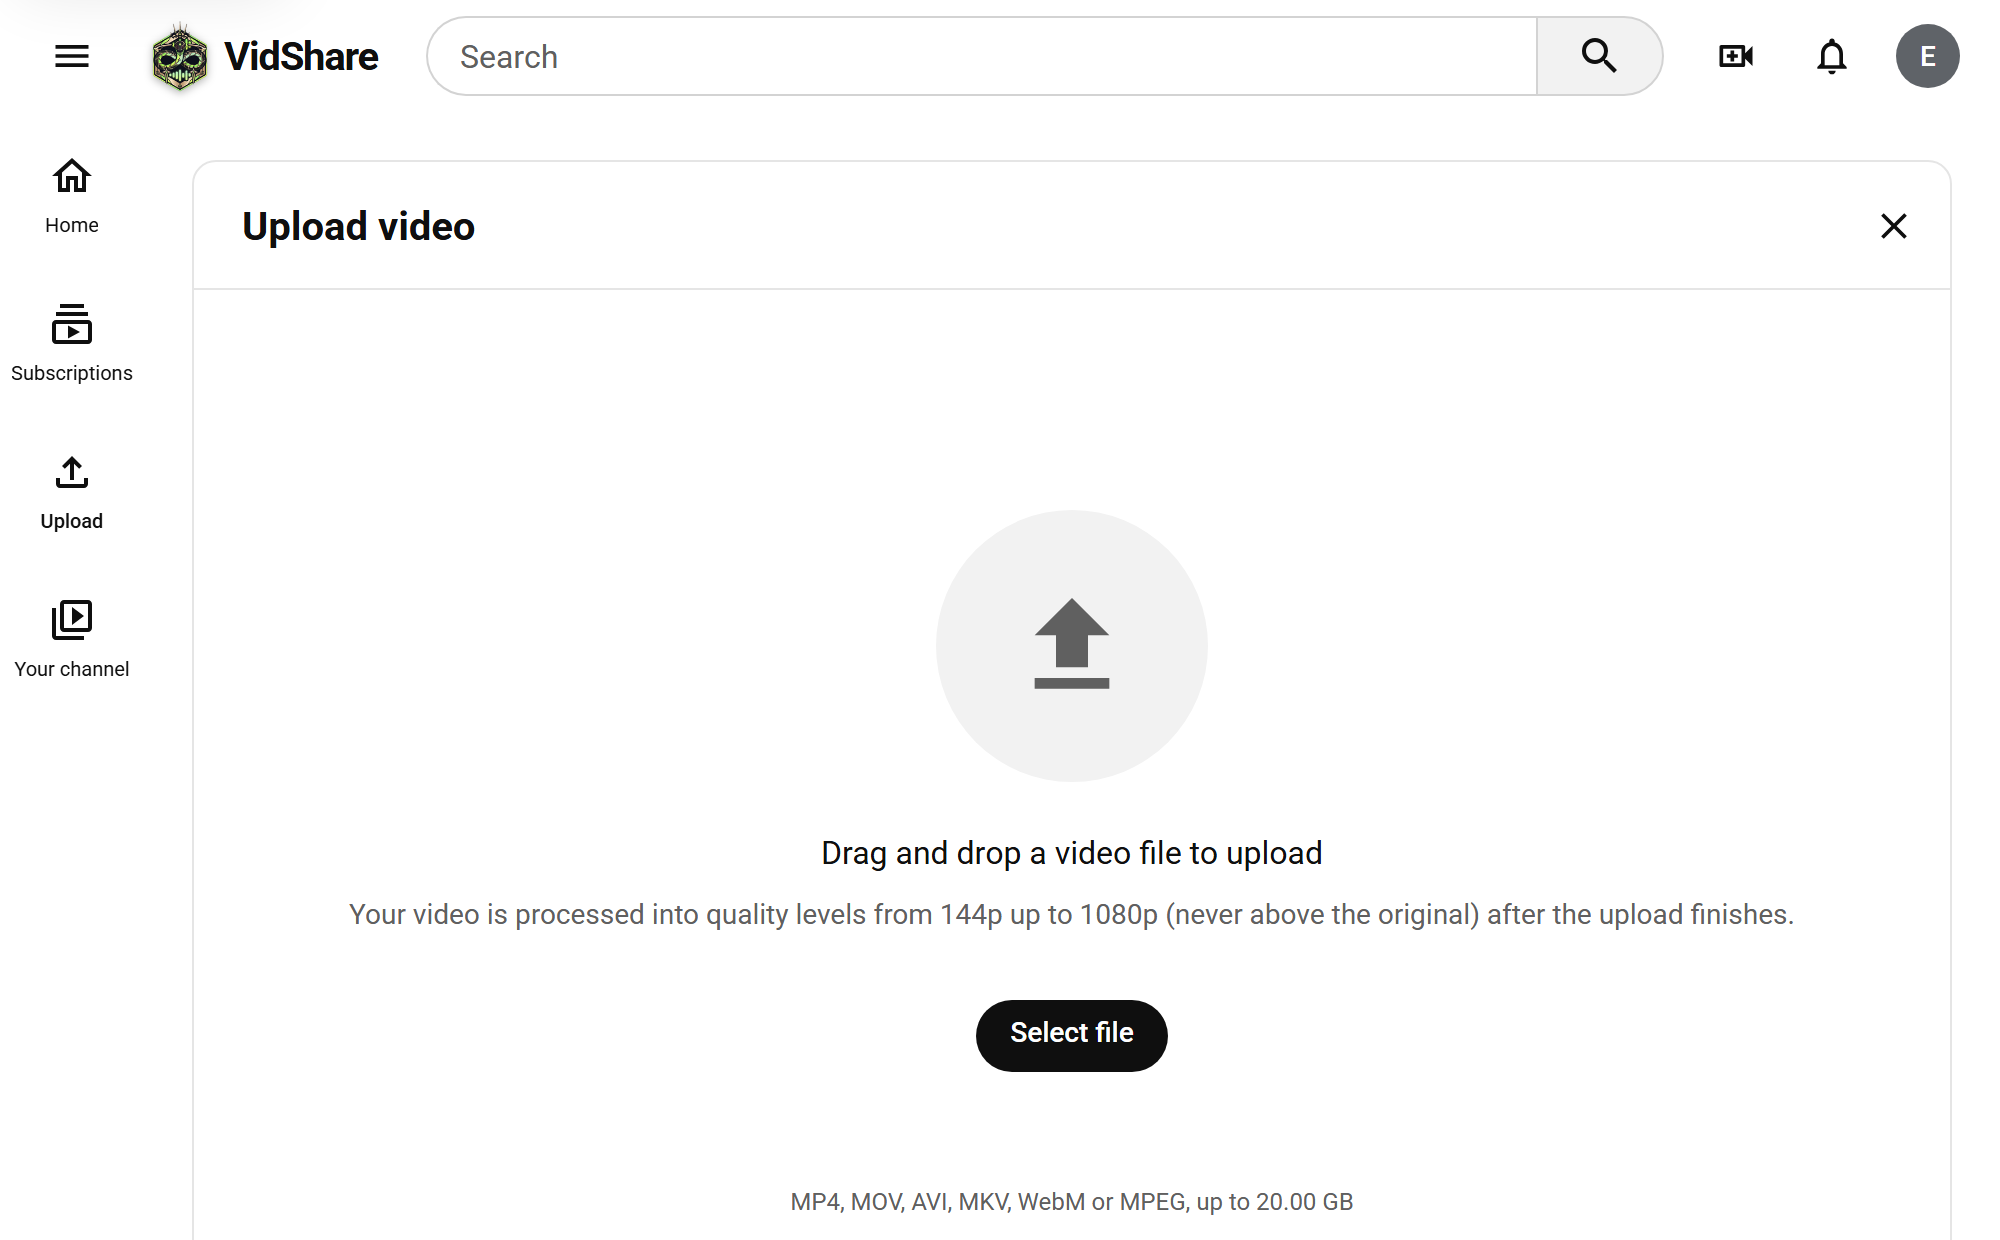
\includegraphics[width=\textwidth]{images/ui-upload.png}
\caption{\textit{Upload page}}
\label{fig:ui-upload}
\end{figure}

\begin{figure}[htbp]
\centering
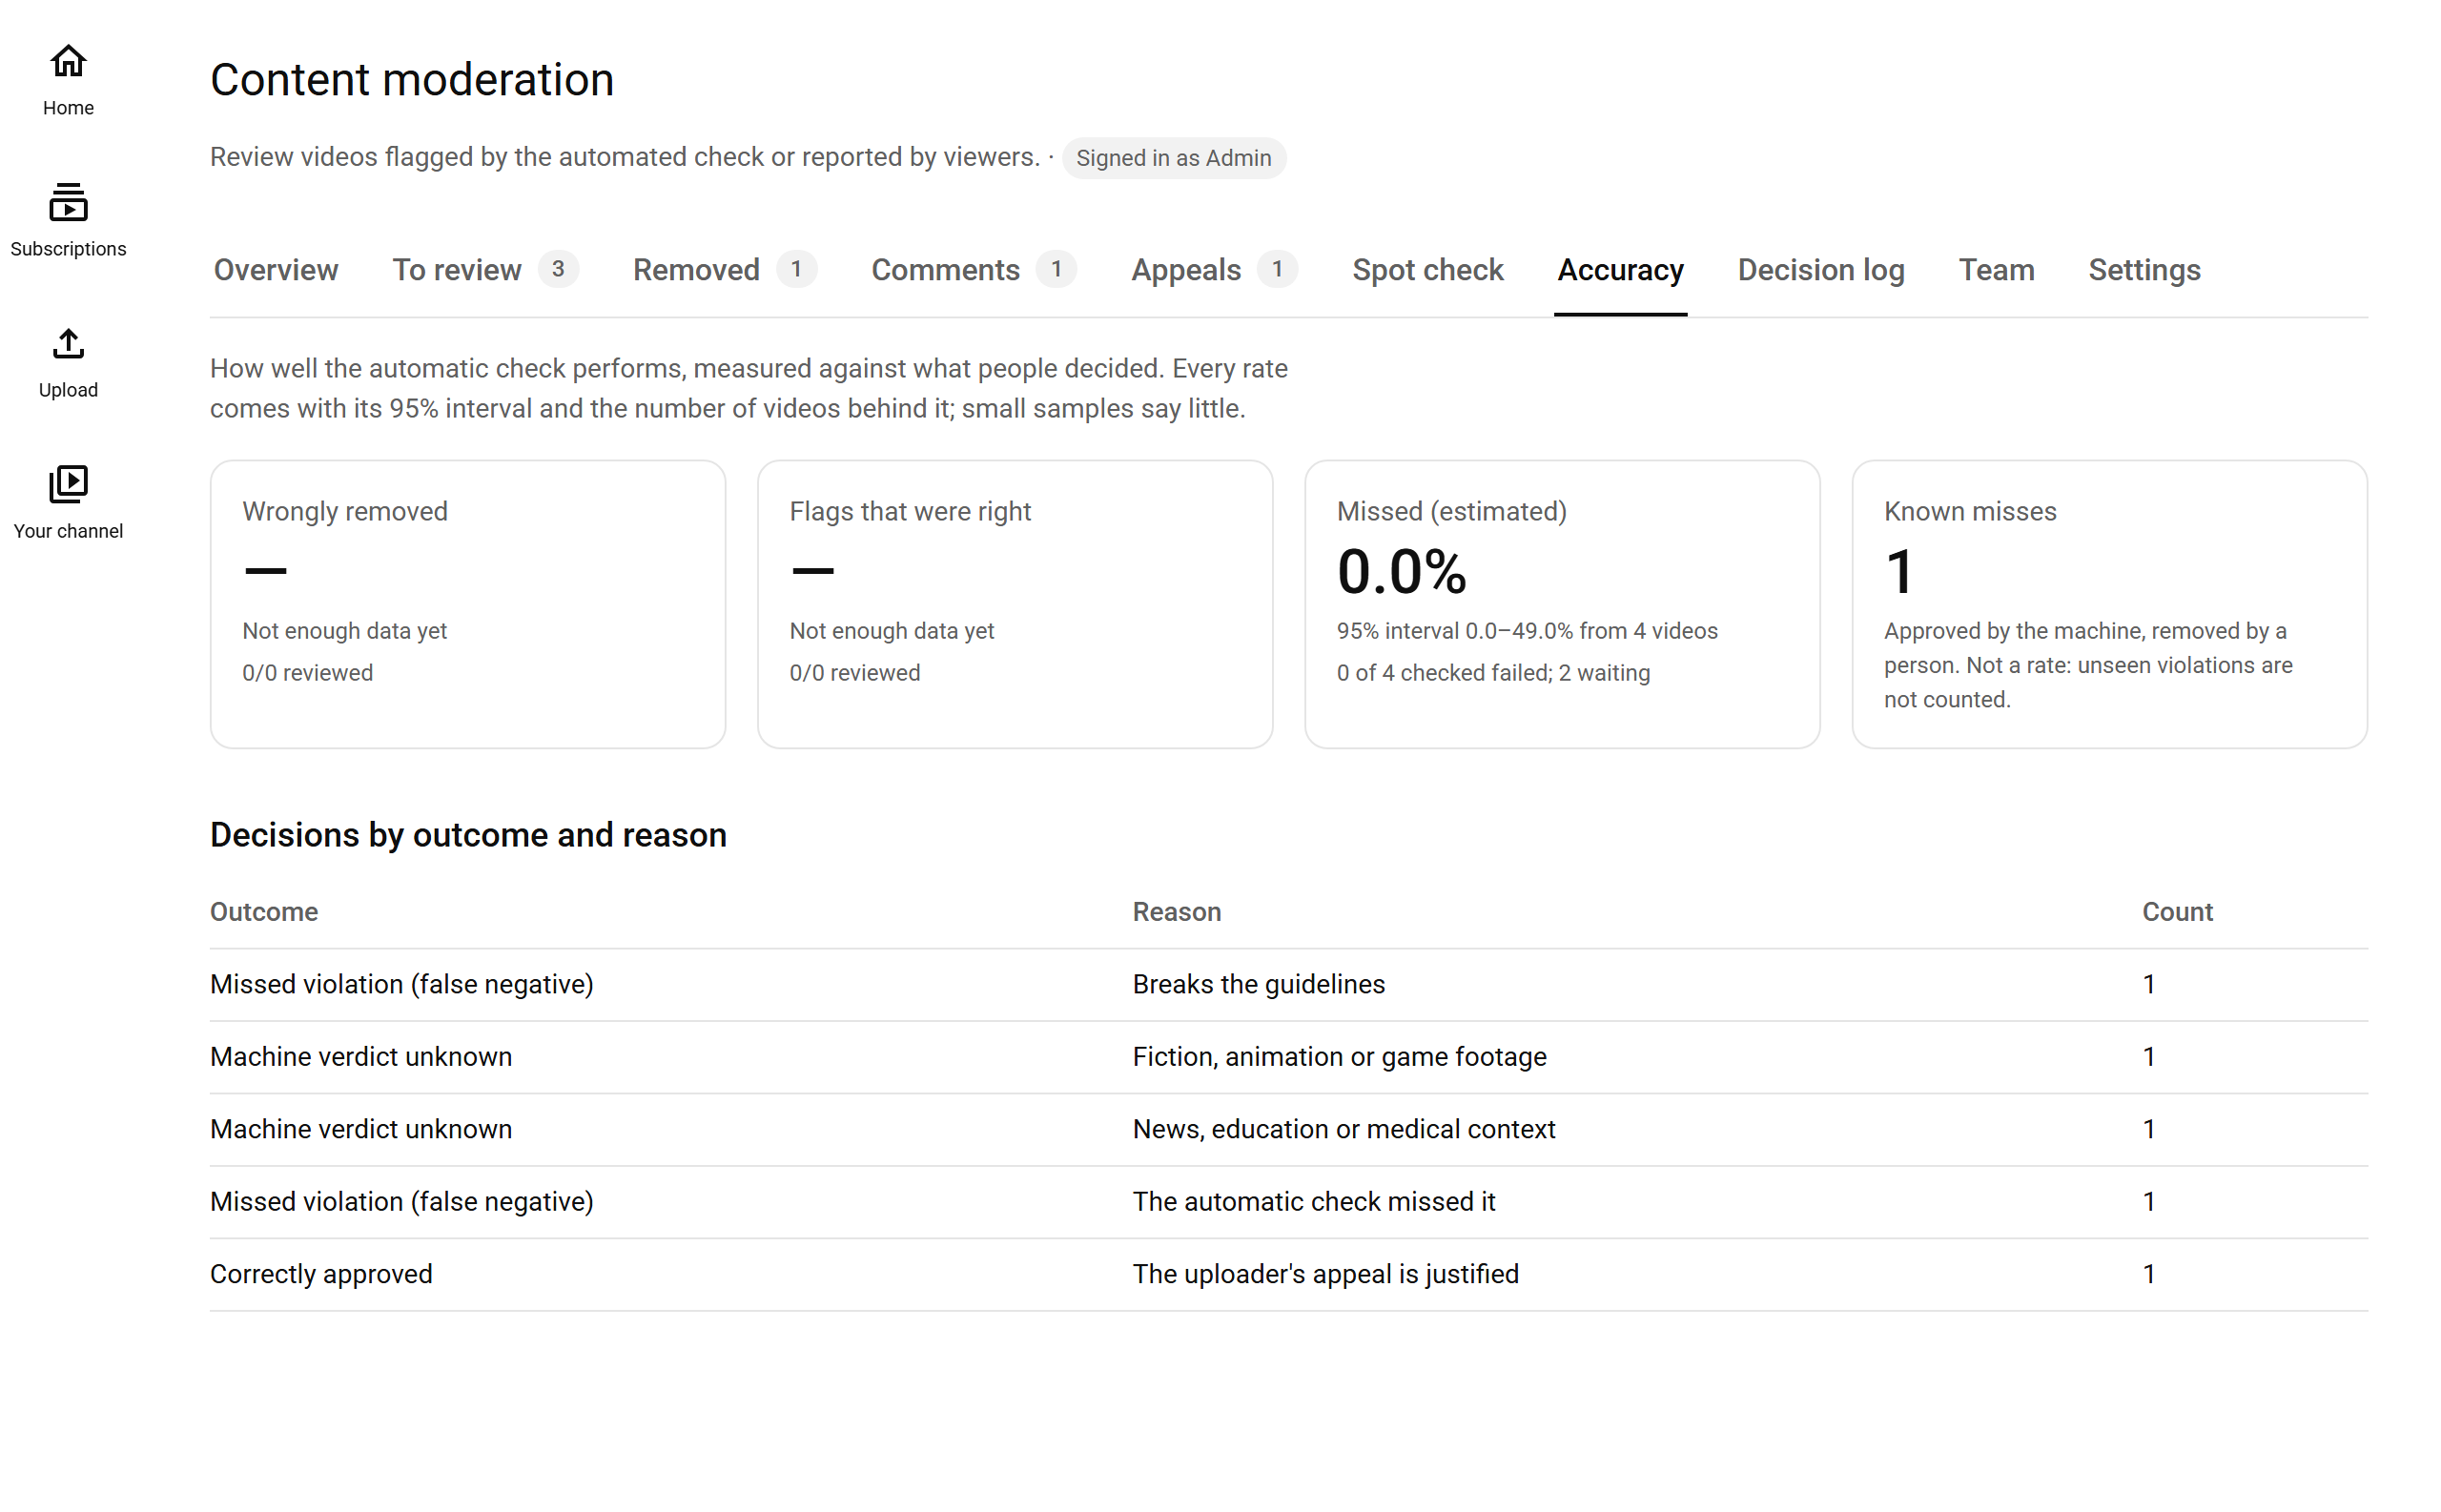
\includegraphics[width=\textwidth]{images/ui-console-accuracy.png}
\caption{\textit{Accuracy tab of the staff console}}
\label{fig:ui-console}
\end{figure}

Figure~\ref{fig:ui-search} shows a search typed without Vietnamese diacritics. The query
\emph{xay lang} finds the title \emph{xây làng}, because the search index folds diacritics on both
sides (Section~\ref{sec:database-design}). Figure~\ref{fig:ui-channel} shows the page of a channel,
with its handle, its subscriber count and its videos.

\begin{figure}[htbp]
\centering
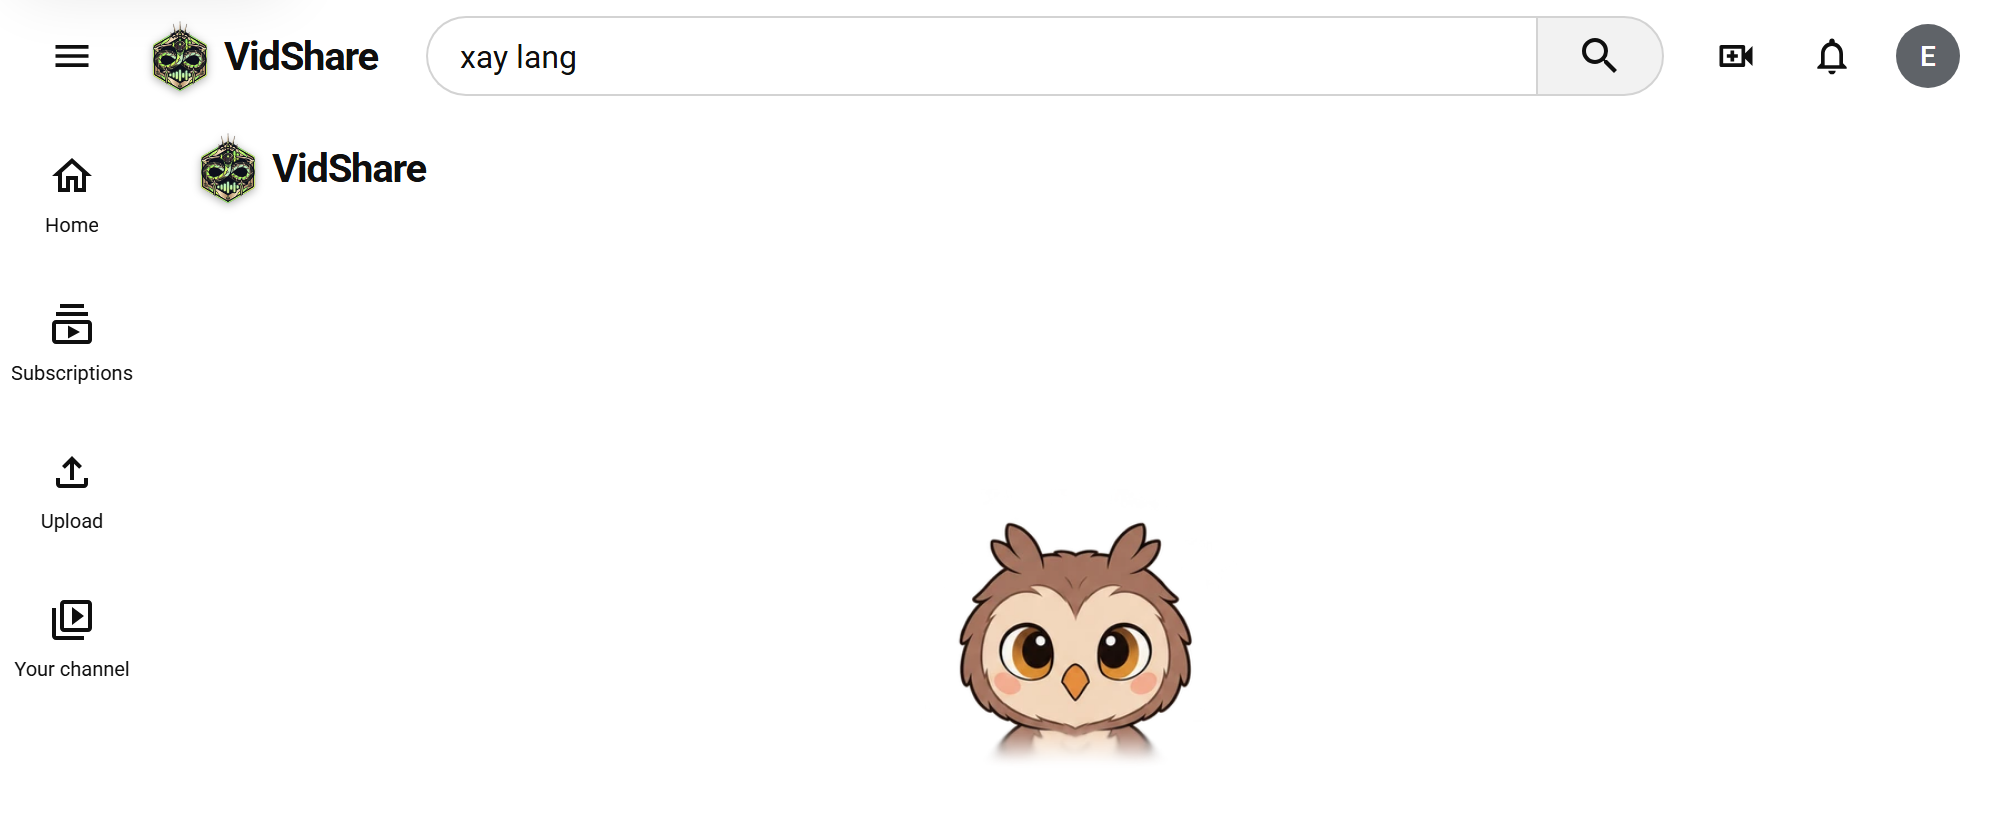
\includegraphics[width=\textwidth]{images/ui-search.png}
\caption{\textit{Search results for a query typed without diacritics}}
\label{fig:ui-search}
\end{figure}

\begin{figure}[htbp]
\centering
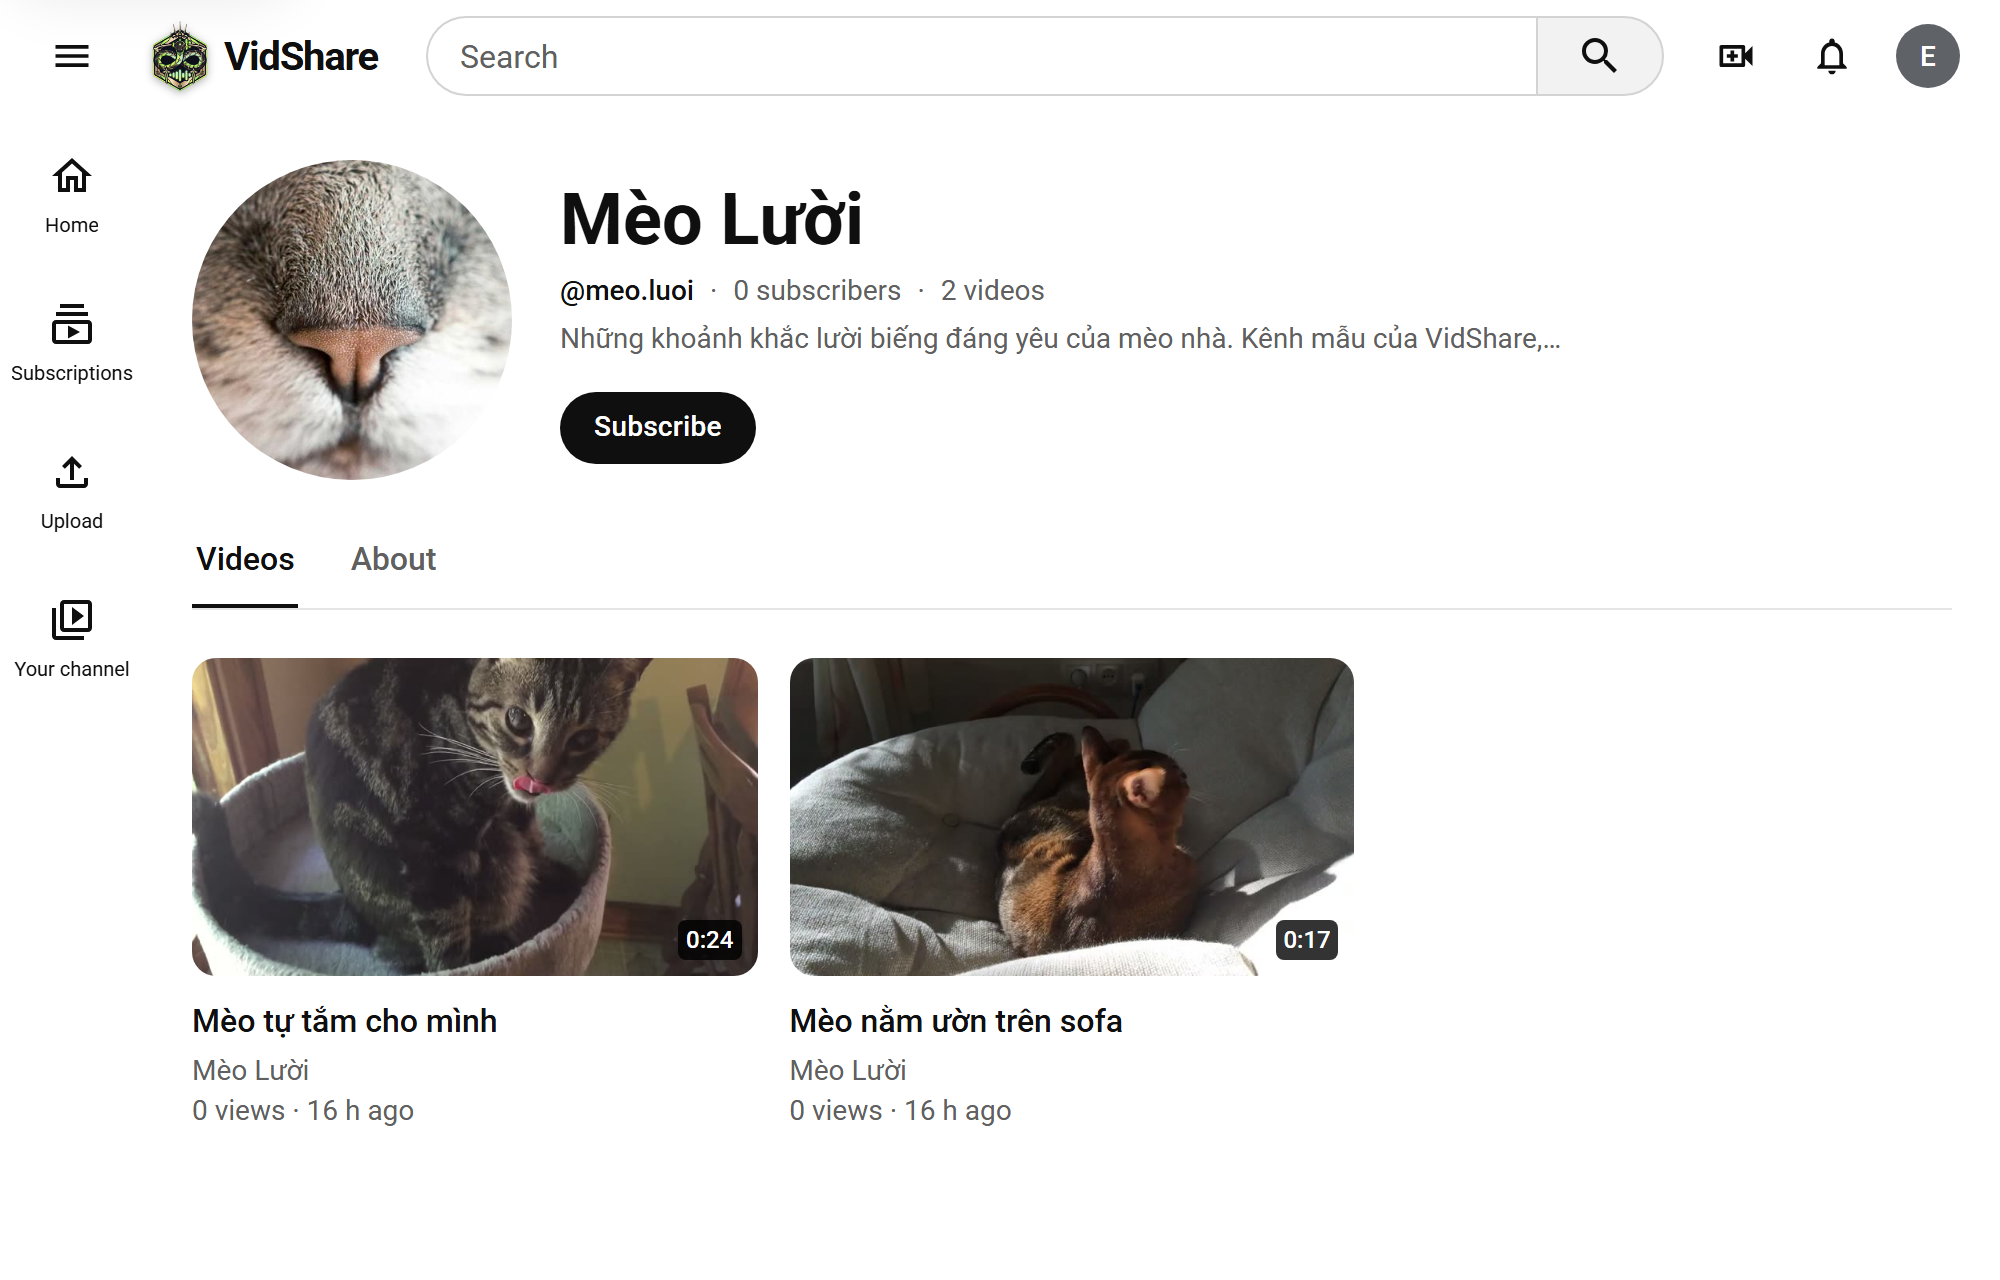
\includegraphics[width=\textwidth]{images/ui-channel.png}
\caption{\textit{Channel page}}
\label{fig:ui-channel}
\end{figure}

The other tabs of the console carry the moderation work of Section~\ref{sec:screening-design}.
The activity they show was produced on production with the sample accounts: comments and reports
from viewers, two removals of benchmark clips, one appeal upheld and one still open.
Figure~\ref{fig:ui-review} shows the review queue. A video enters it when screening holds it or when
viewers report it; its image stays blurred until the reviewer asks to see it, and the open reports
can be expanded before the video is kept or removed. Figure~\ref{fig:ui-comments} lists the reported
comments, most reported first: keeping one closes its reports, and removing it deletes it with its
replies. An appeal against a removal appears in the tab of Figure~\ref{fig:ui-appeals} with the
creator's message, a field for the reply and the choice between restoring the video and keeping it
removed. Figure~\ref{fig:ui-audit} shows the spot check, a random sample of videos that screening
approved, each marked pass or fail; the share that fails is the estimate of missed violations in
Figure~\ref{fig:ui-console}. Every decision joins the log of Figure~\ref{fig:ui-events} with the
person, the reason and the outcome measured against the verdict of the machine, and a second view of
the same tab lists the changes of role.

\begin{figure}[htbp]
\centering
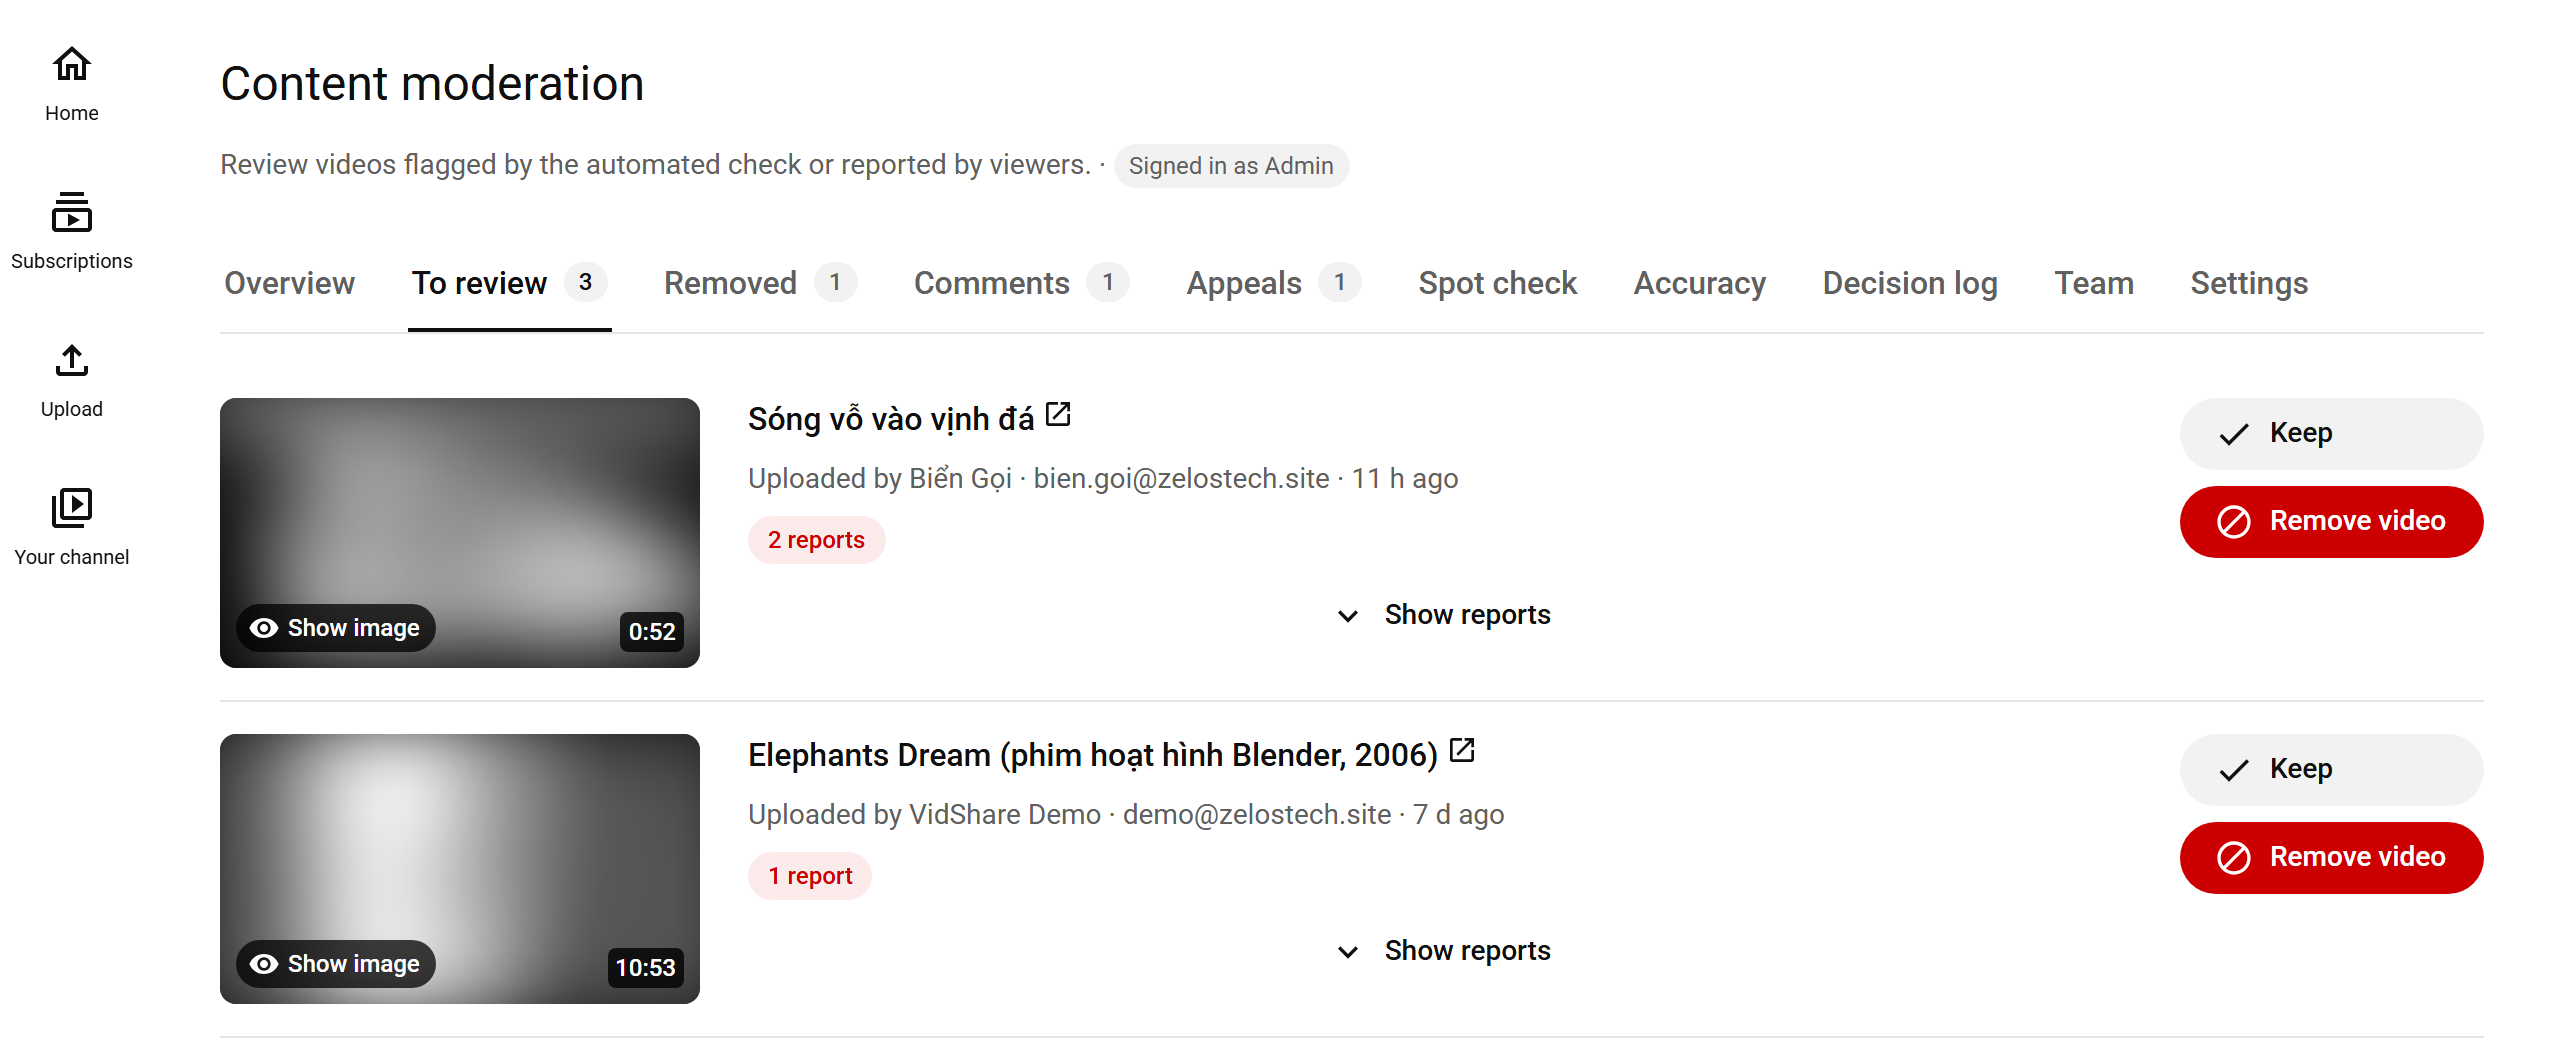
\includegraphics[width=\textwidth]{images/ui-admin-review.png}
\caption{\textit{Review queue of the staff console with videos reported by viewers}}
\label{fig:ui-review}
\end{figure}

\begin{figure}[htbp]
\centering
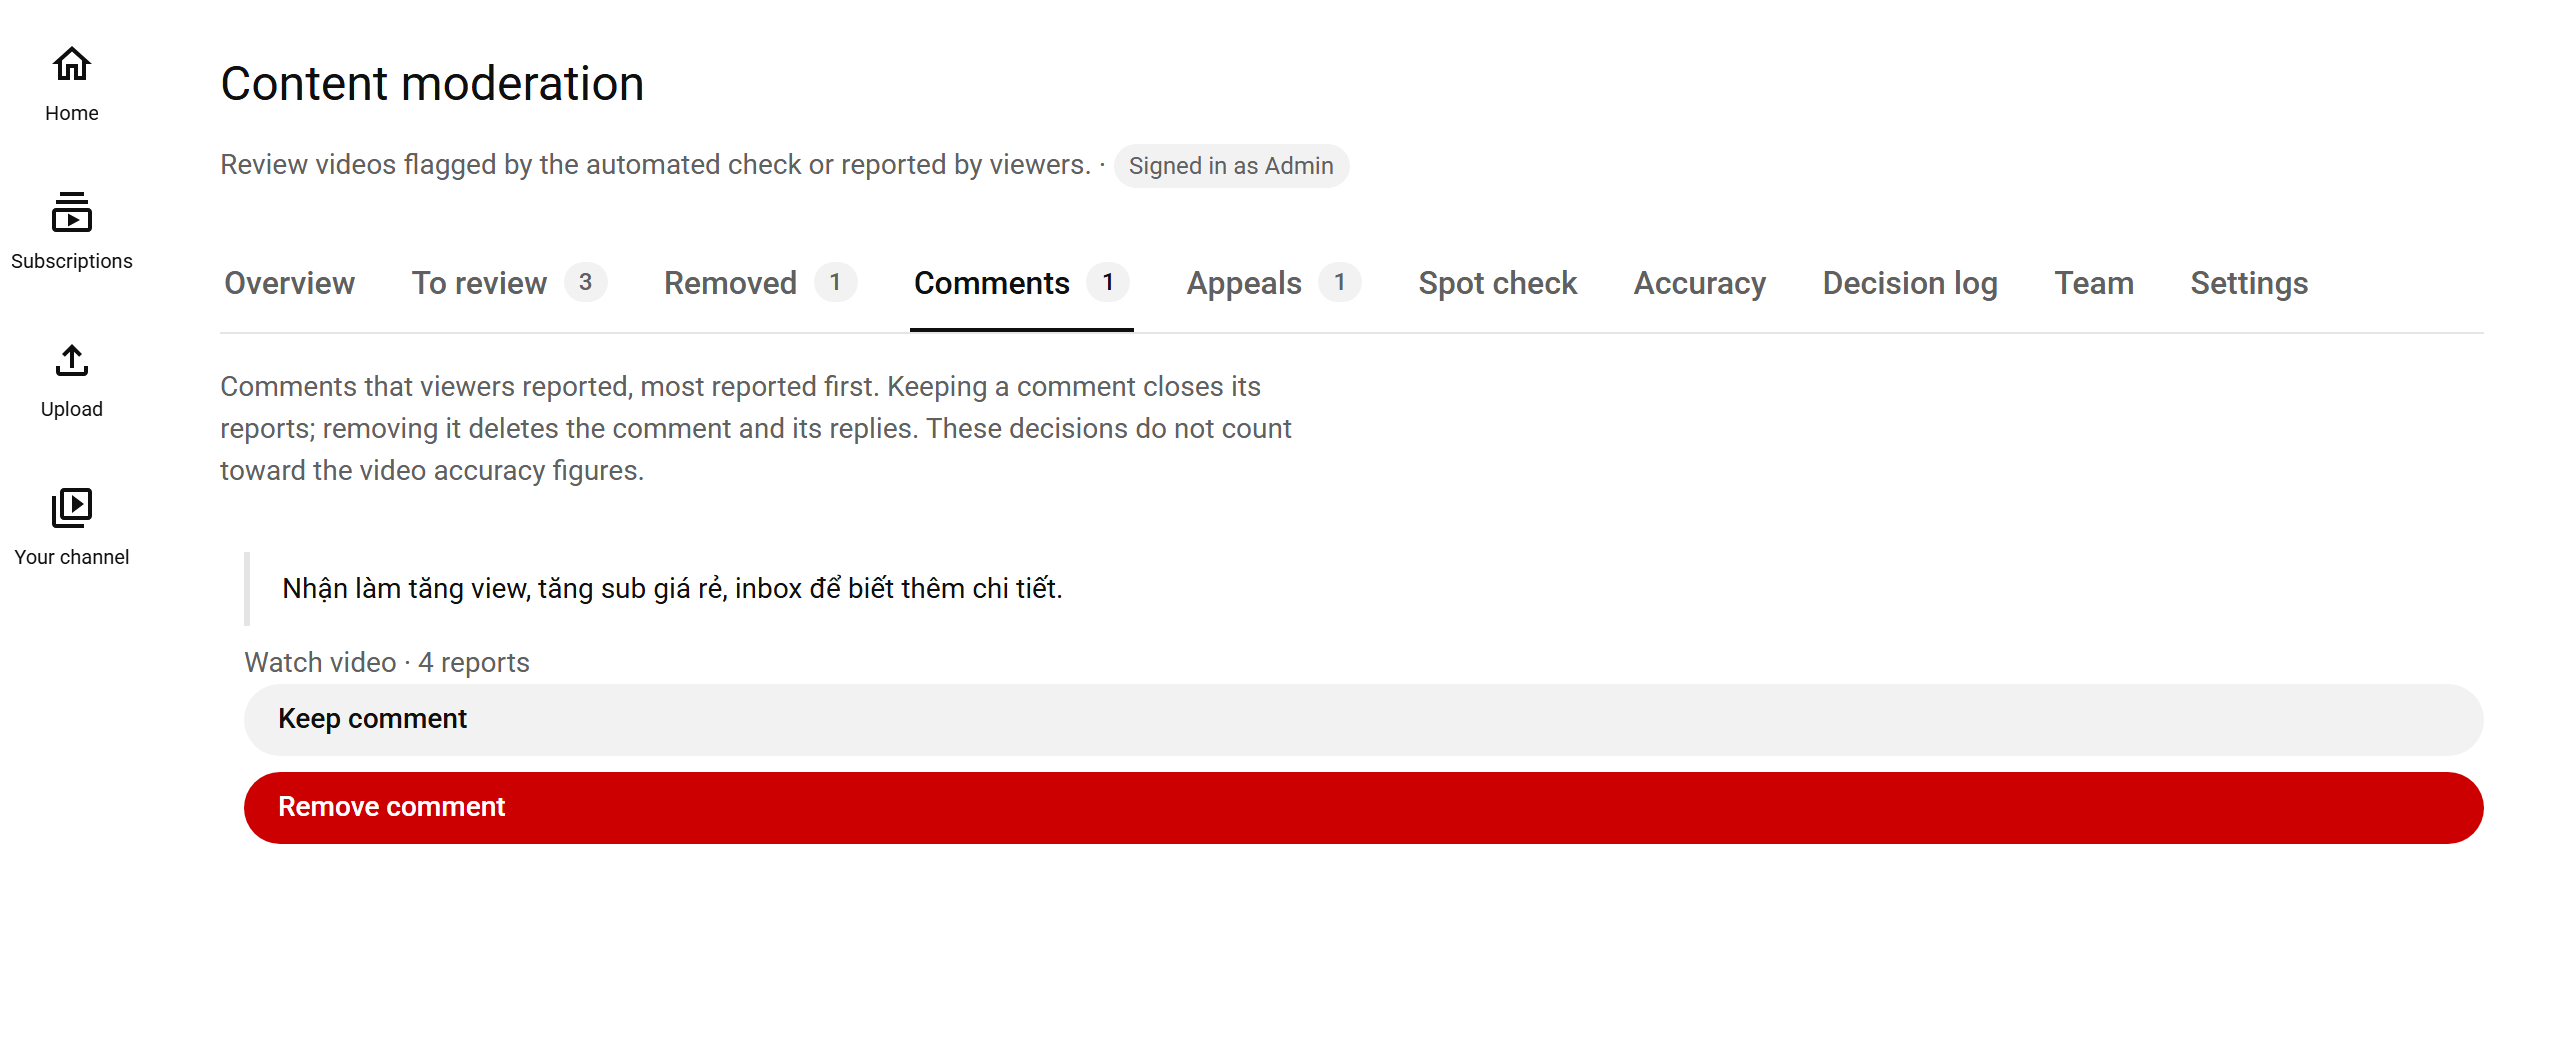
\includegraphics[width=\textwidth]{images/ui-admin-comments.png}
\caption{\textit{Reported comments in the staff console}}
\label{fig:ui-comments}
\end{figure}

\begin{figure}[htbp]
\centering
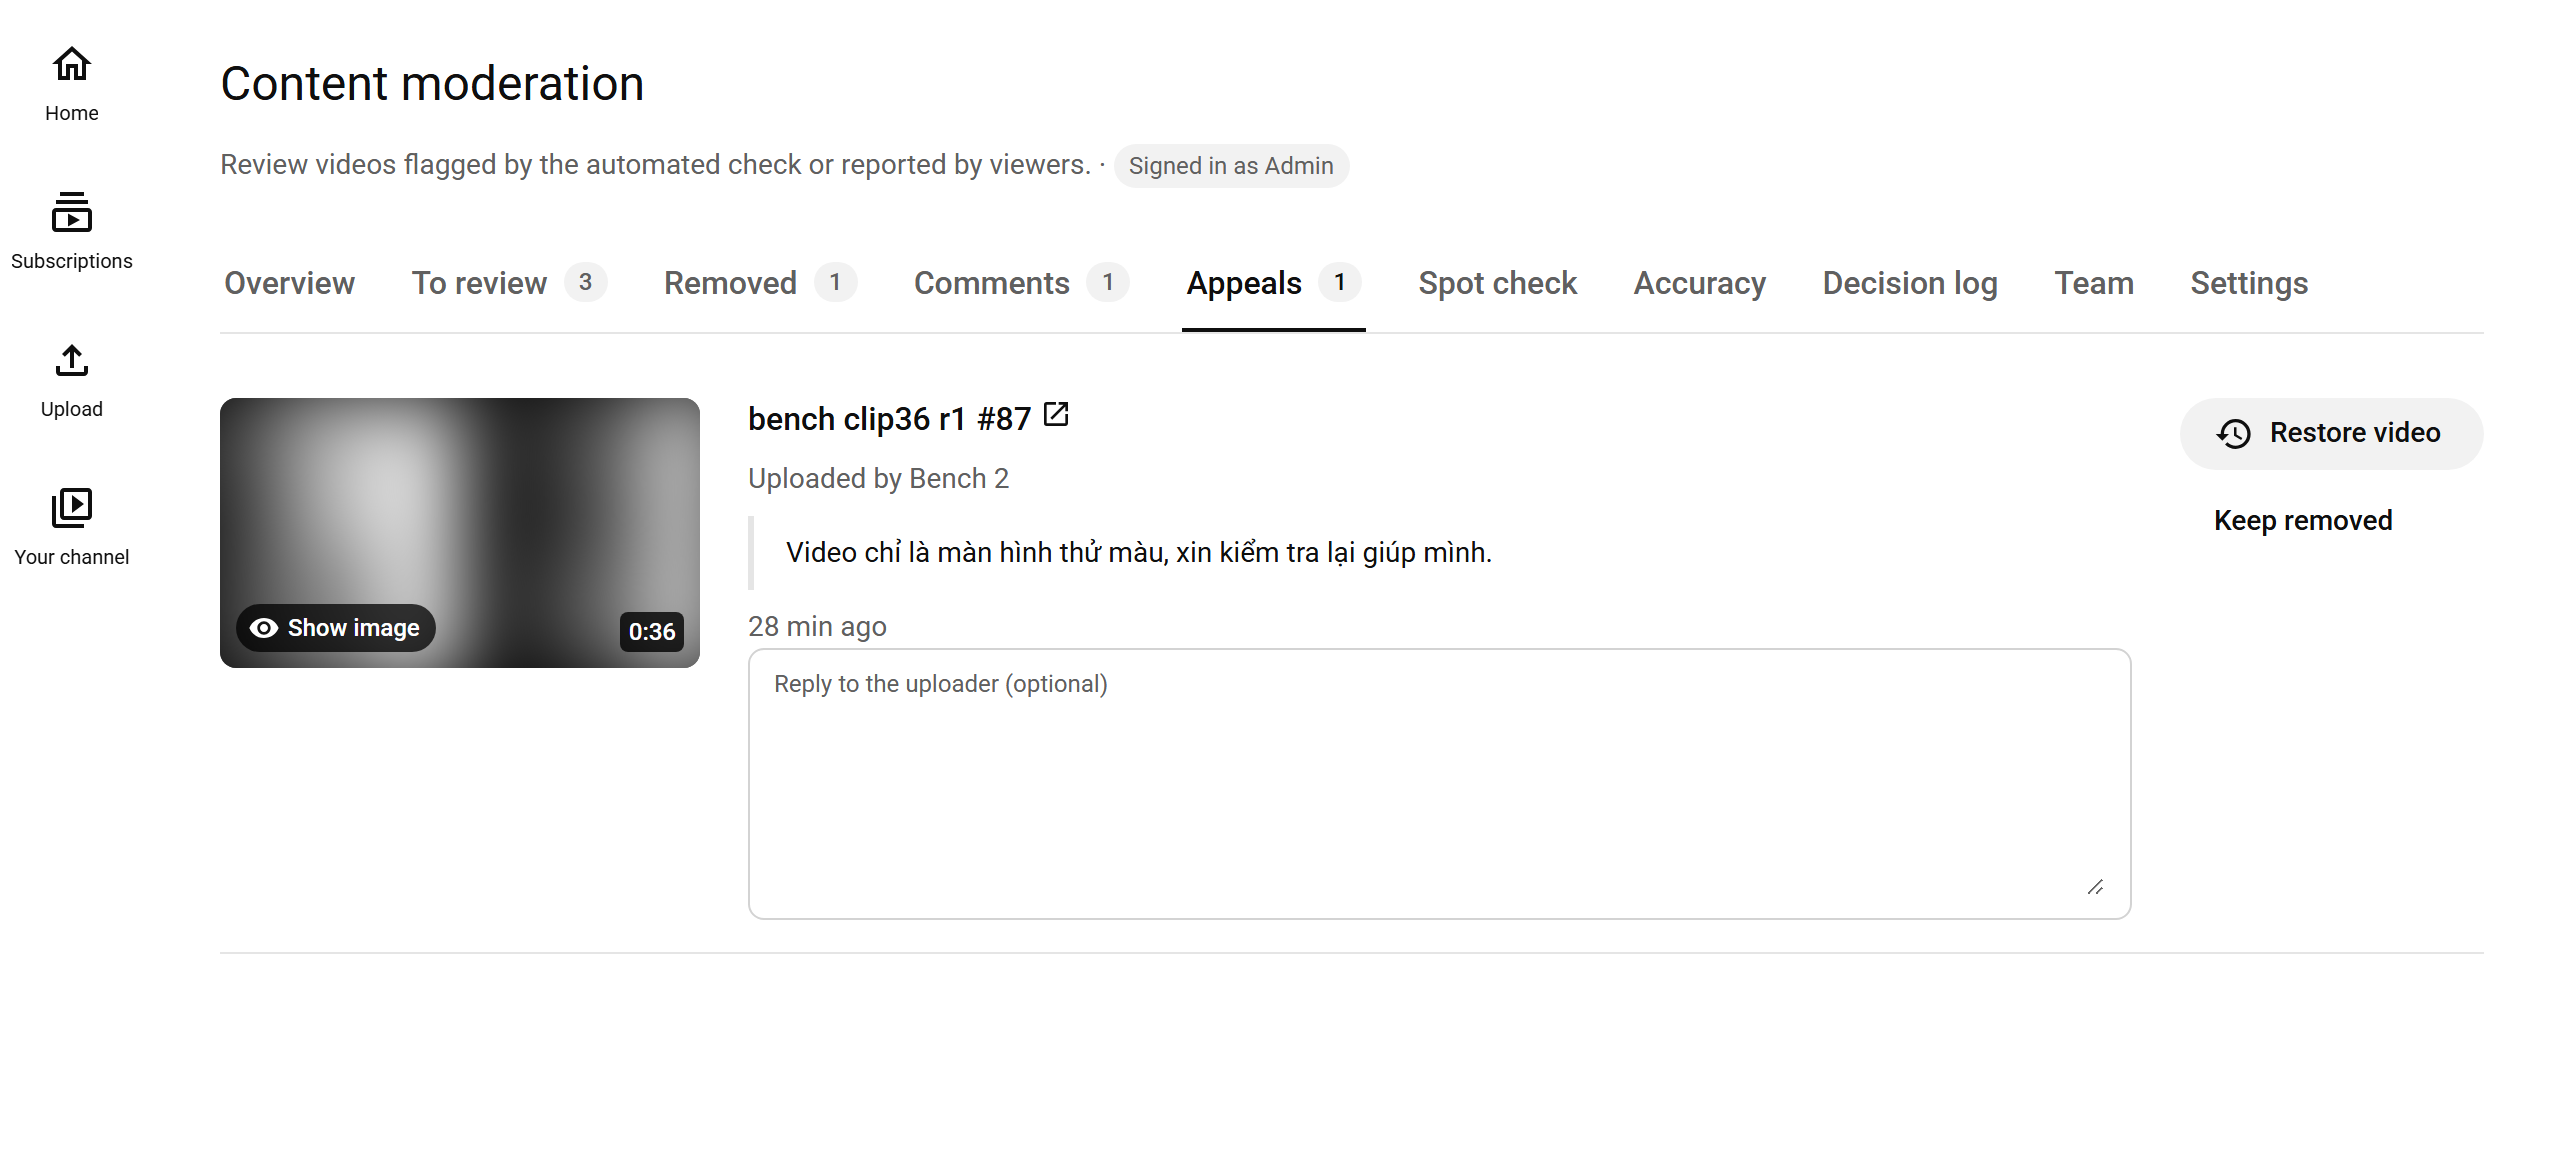
\includegraphics[width=\textwidth]{images/ui-admin-appeals.png}
\caption{\textit{Open appeal of a creator against a removal}}
\label{fig:ui-appeals}
\end{figure}

\begin{figure}[htbp]
\centering
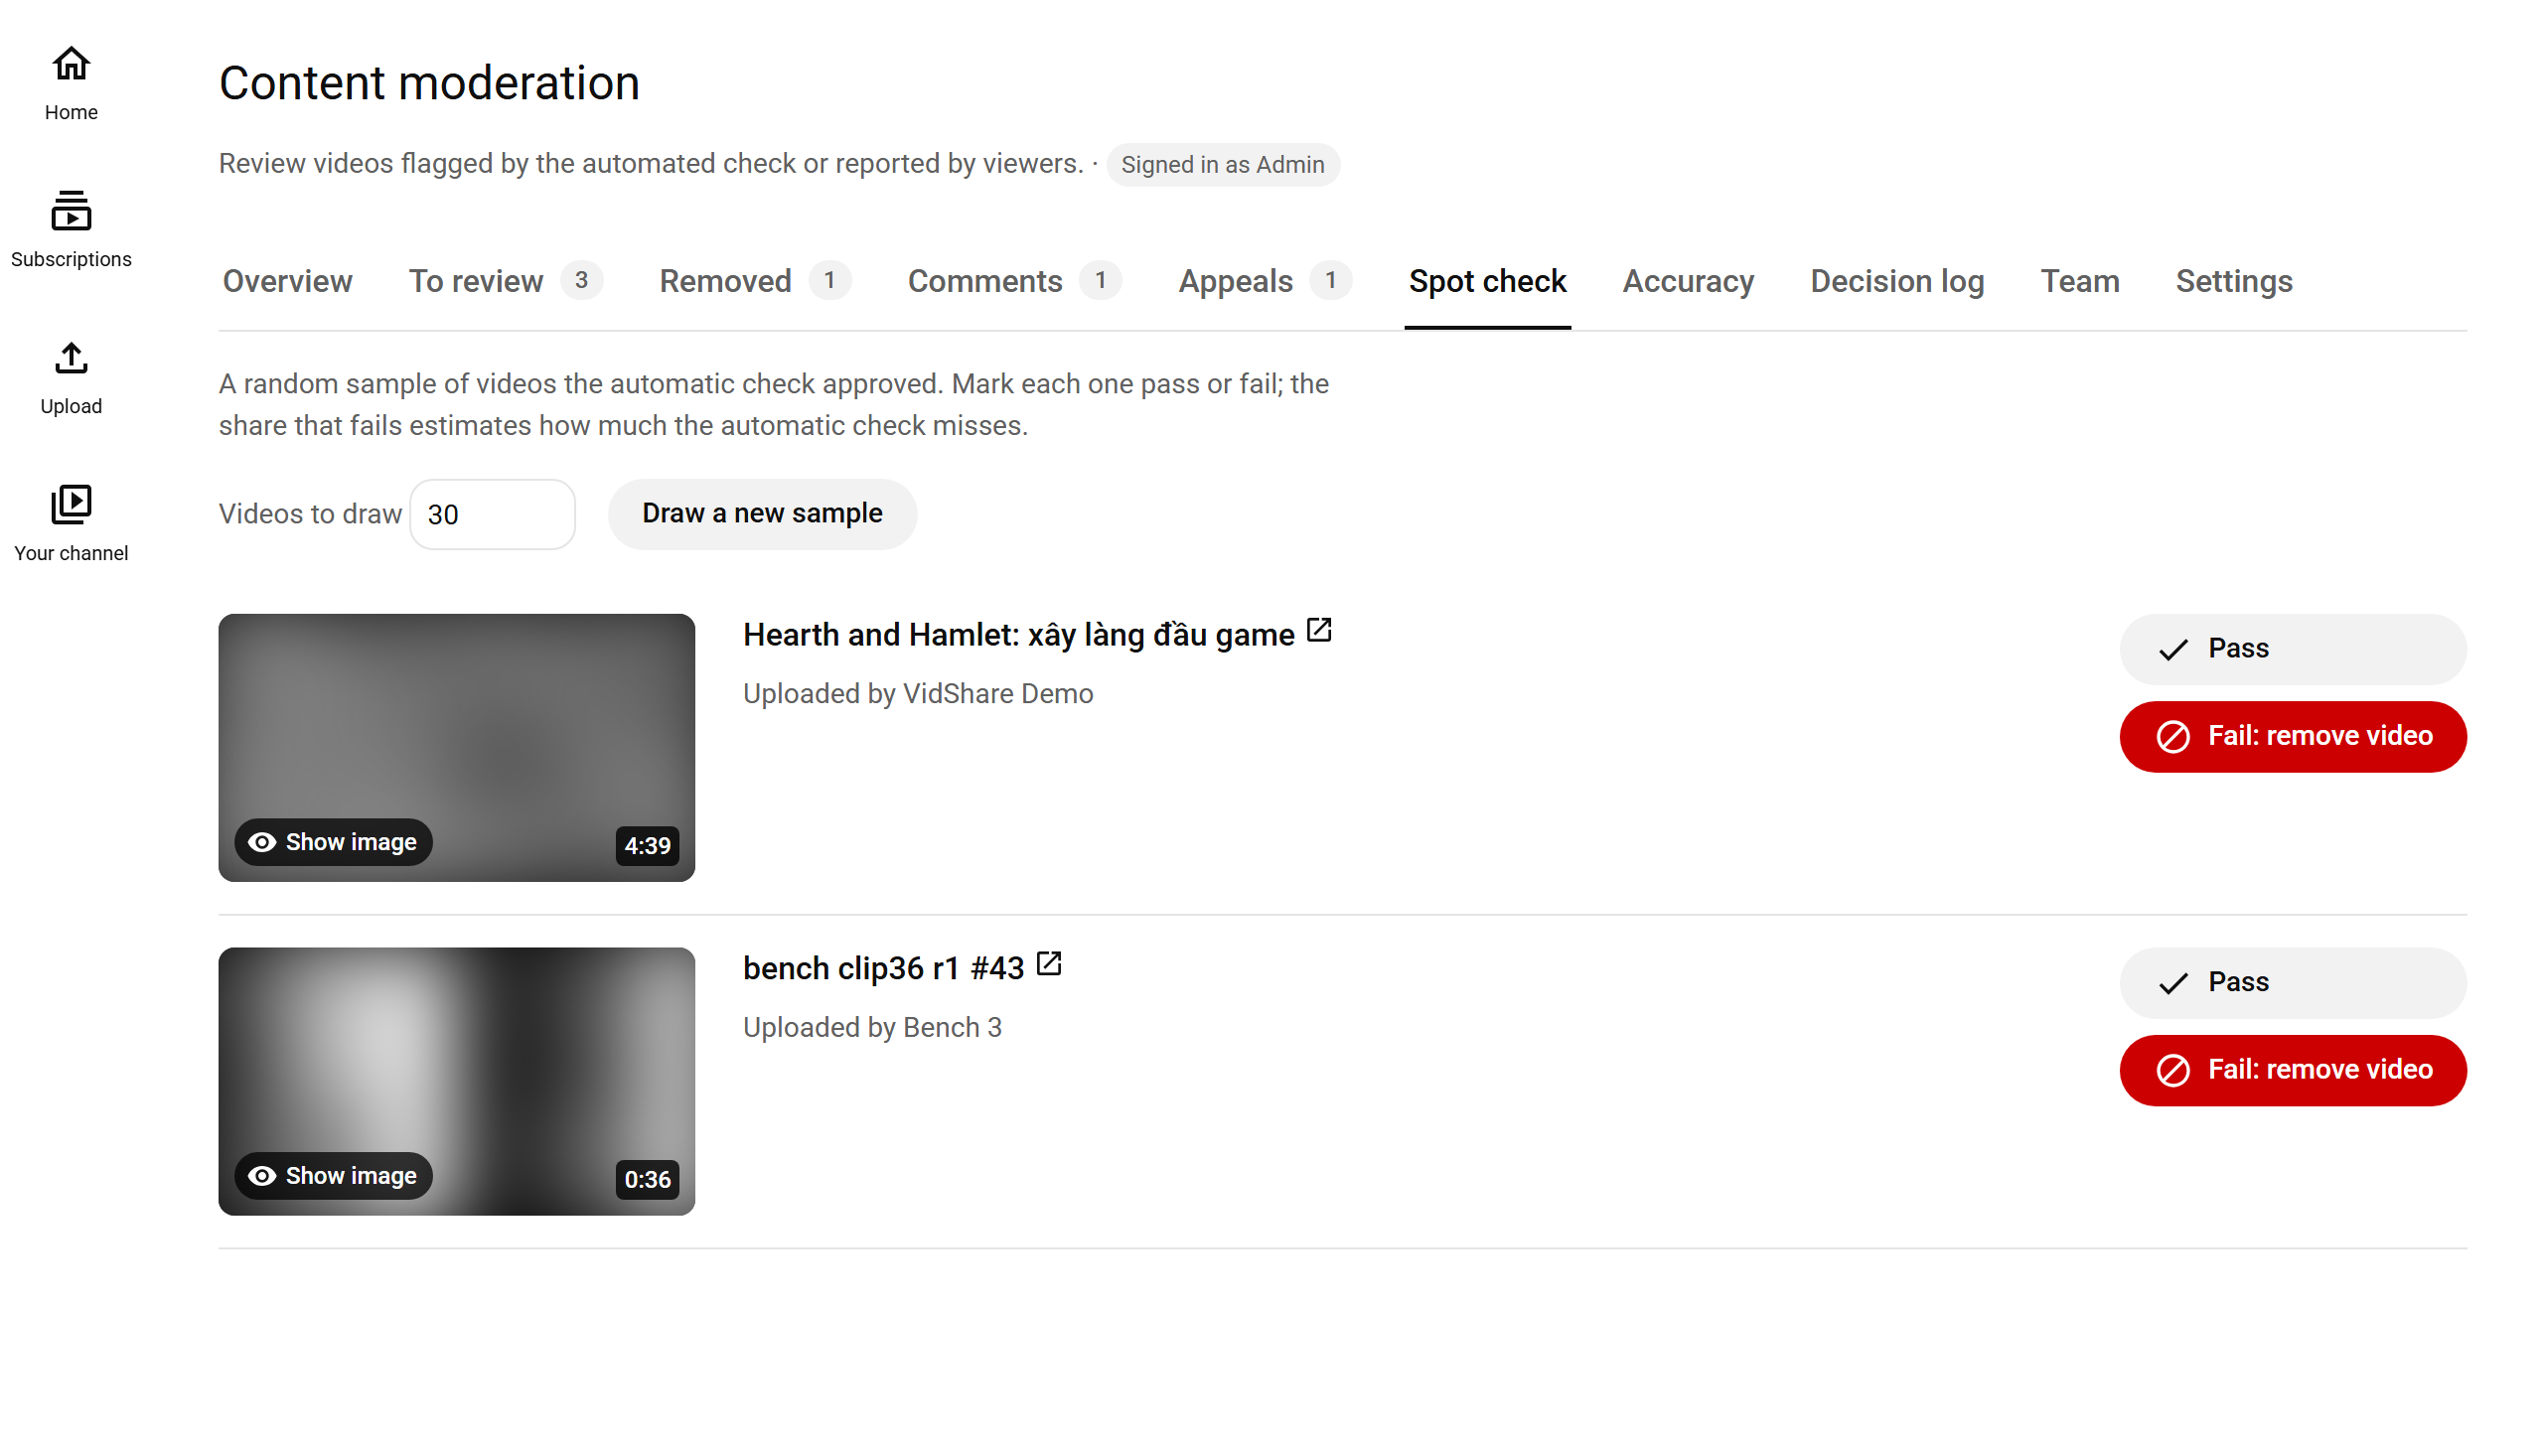
\includegraphics[width=\textwidth]{images/ui-admin-audit.png}
\caption{\textit{Spot check of videos approved by screening}}
\label{fig:ui-audit}
\end{figure}

\begin{figure}[htbp]
\centering
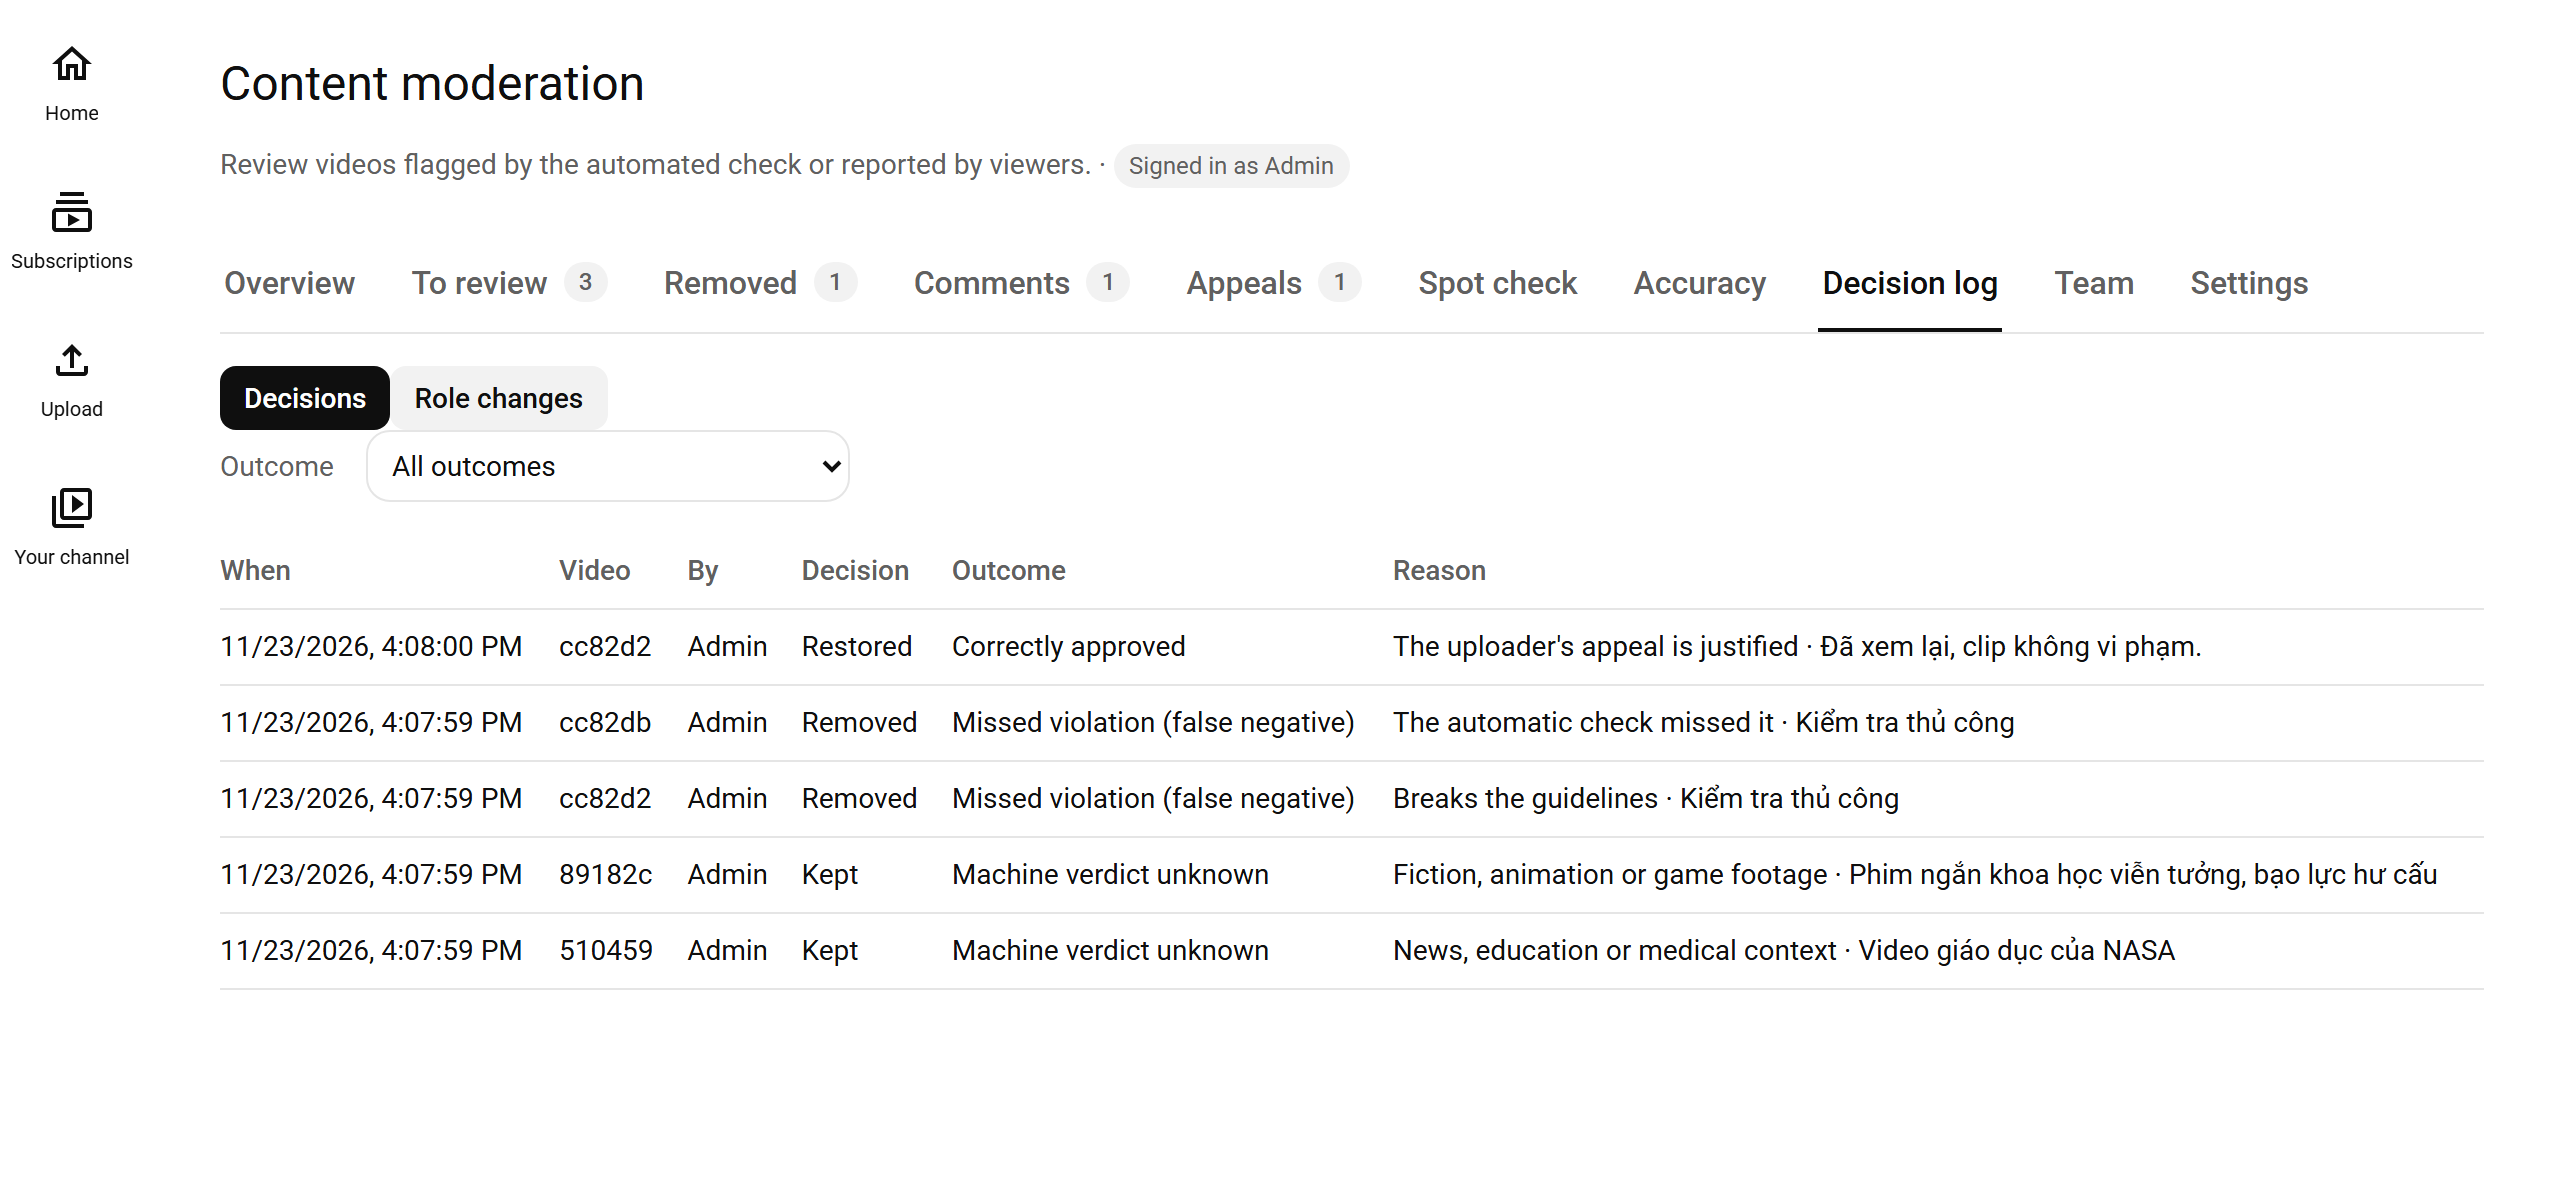
\includegraphics[width=\textwidth]{images/ui-admin-events.png}
\caption{\textit{Decision log of the staff console}}
\label{fig:ui-events}
\end{figure}

Figure~\ref{fig:ui-overview} shows the overview tab that only an administrator sees. The tiles count
users and plans, content and processing, screening outcomes, caption minutes and views over the
chosen window, here 30 days, and every account counts, the sample channels and the test accounts
included. Below the tiles, one bar chart per day shows sign-ups, uploads and views, and the same
numbers are available as a table. Figure~\ref{fig:ui-settings} shows the settings tab with the two
switches of Section~\ref{sec:screening-design}: each card states what the service does, what it
costs and whether its value was set in the console or comes from the default of the
infrastructure, and every change asks for confirmation and joins the history below the cards.

\begin{figure}[htbp]
\centering
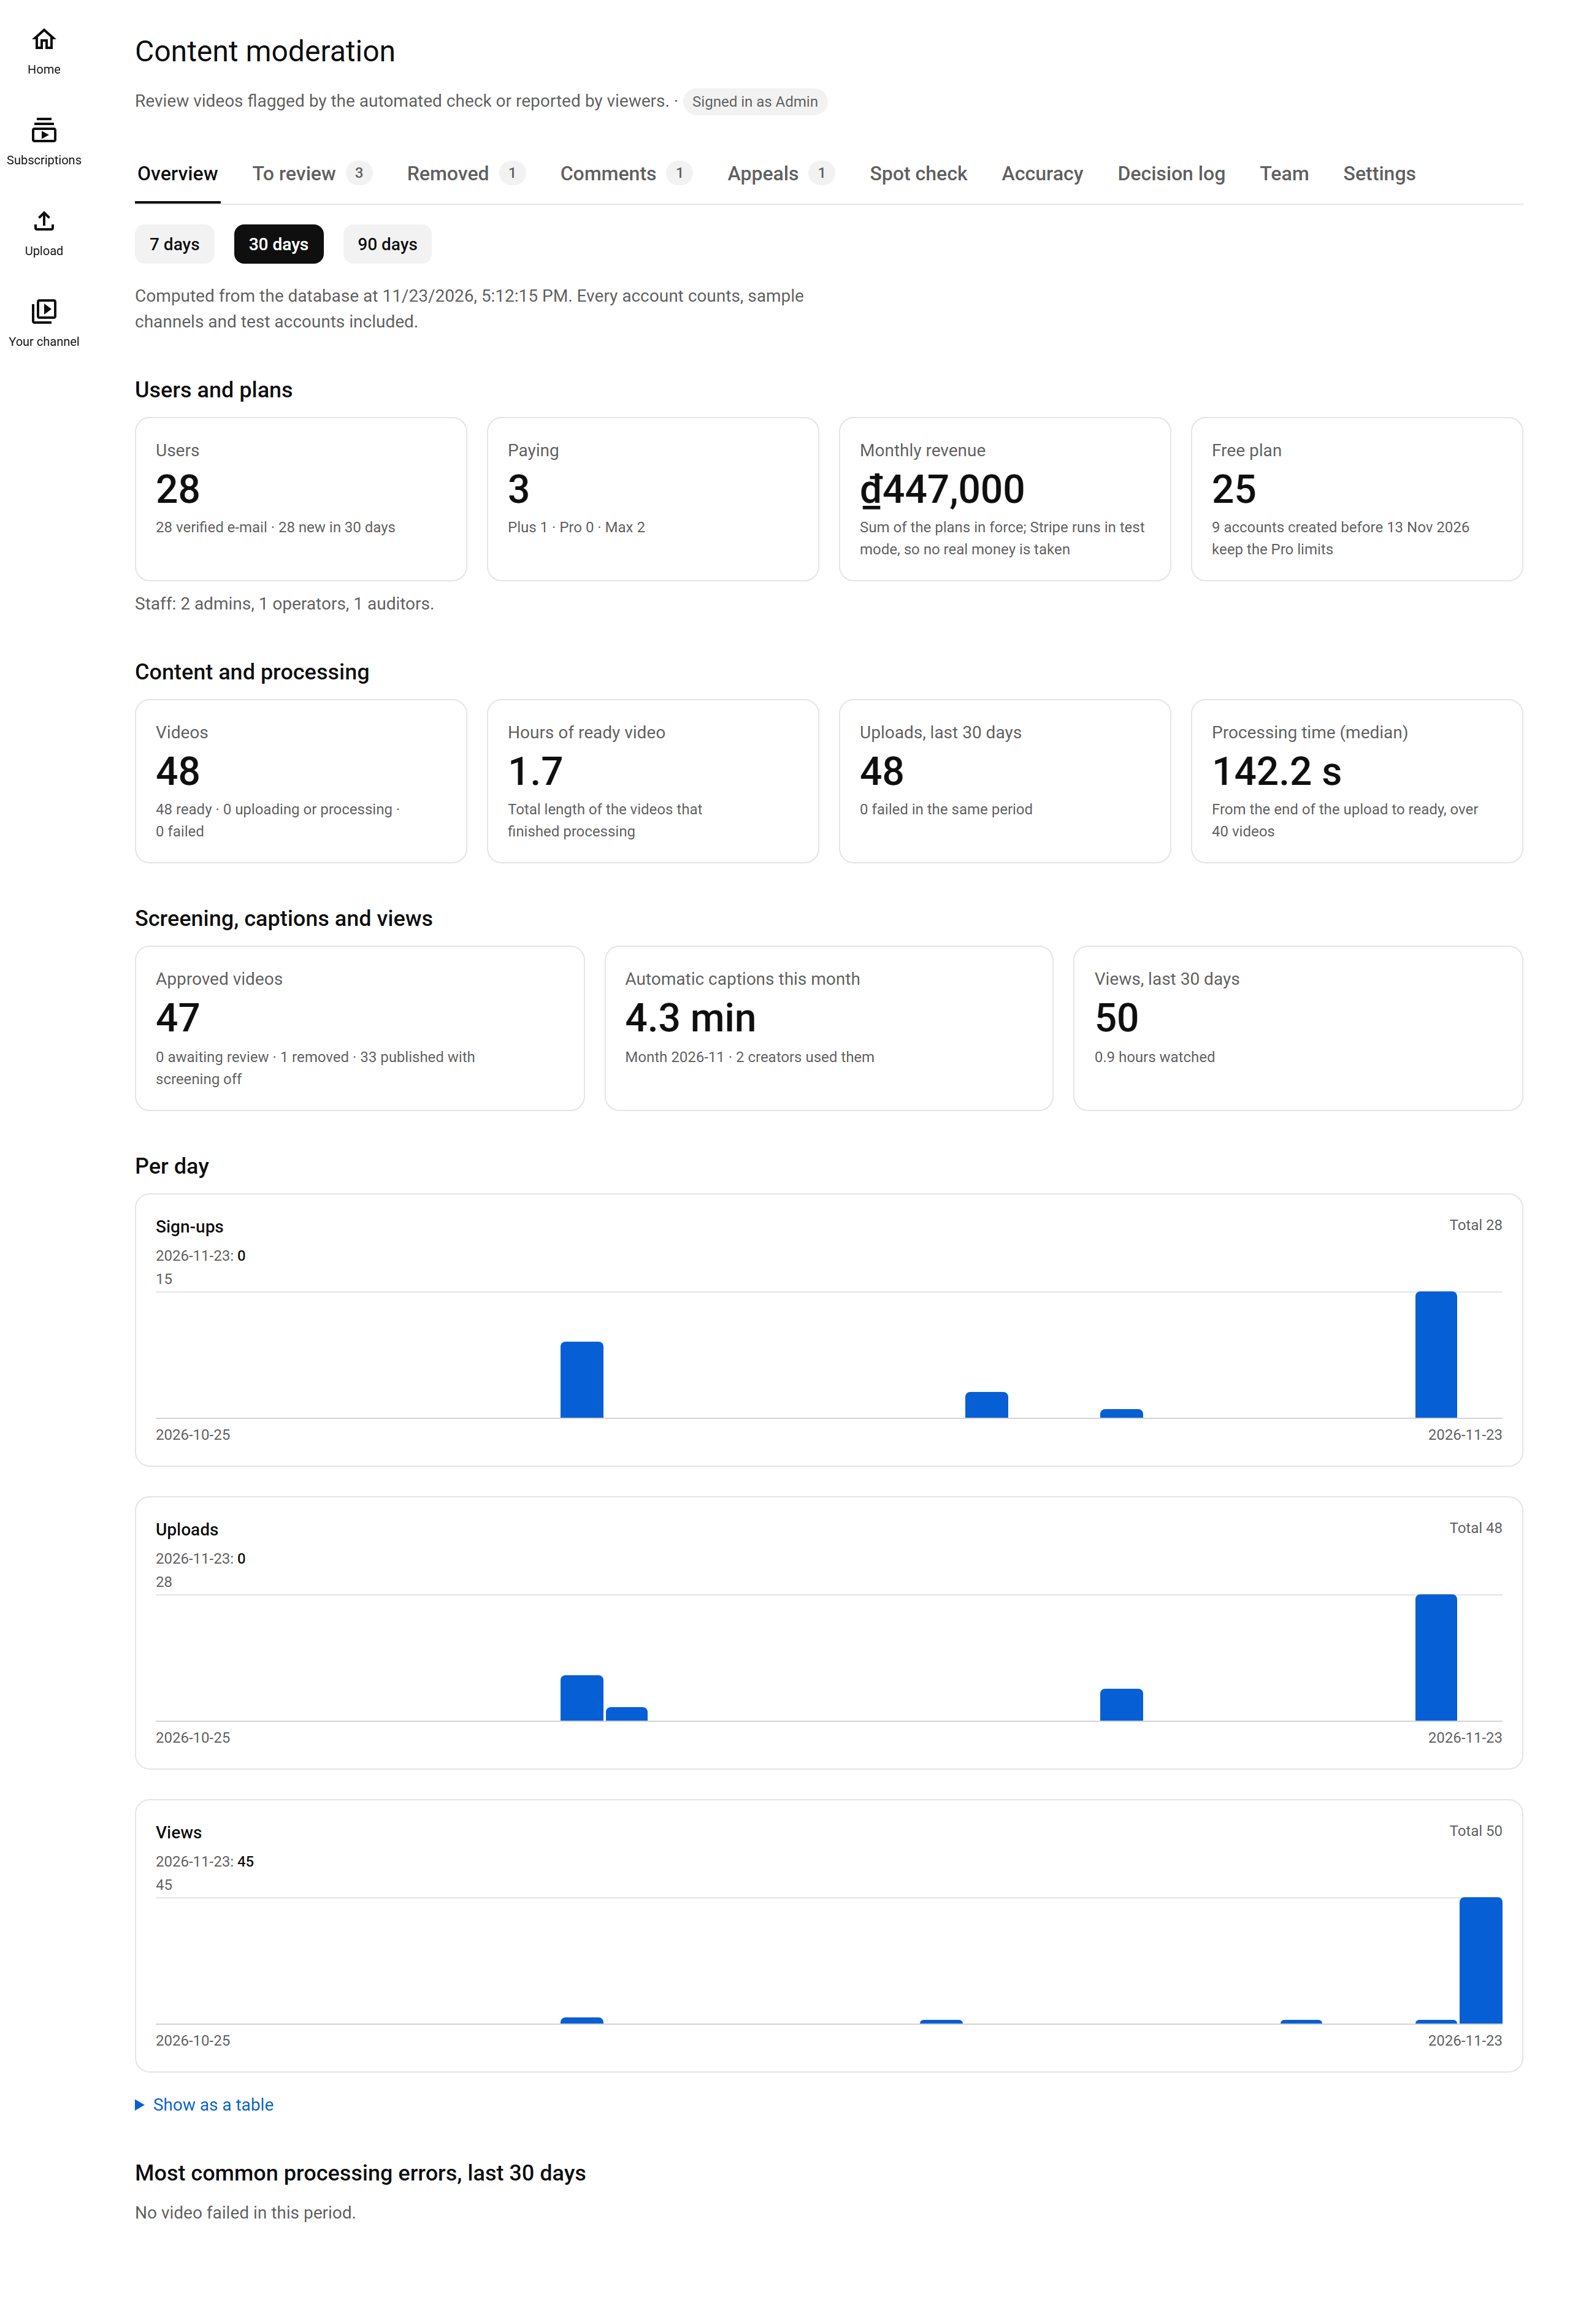
\includegraphics[width=0.8\textwidth]{images/ui-admin-overview.png}
\caption{\textit{Overview tab of the staff console, for administrators}}
\label{fig:ui-overview}
\end{figure}

\begin{figure}[htbp]
\centering
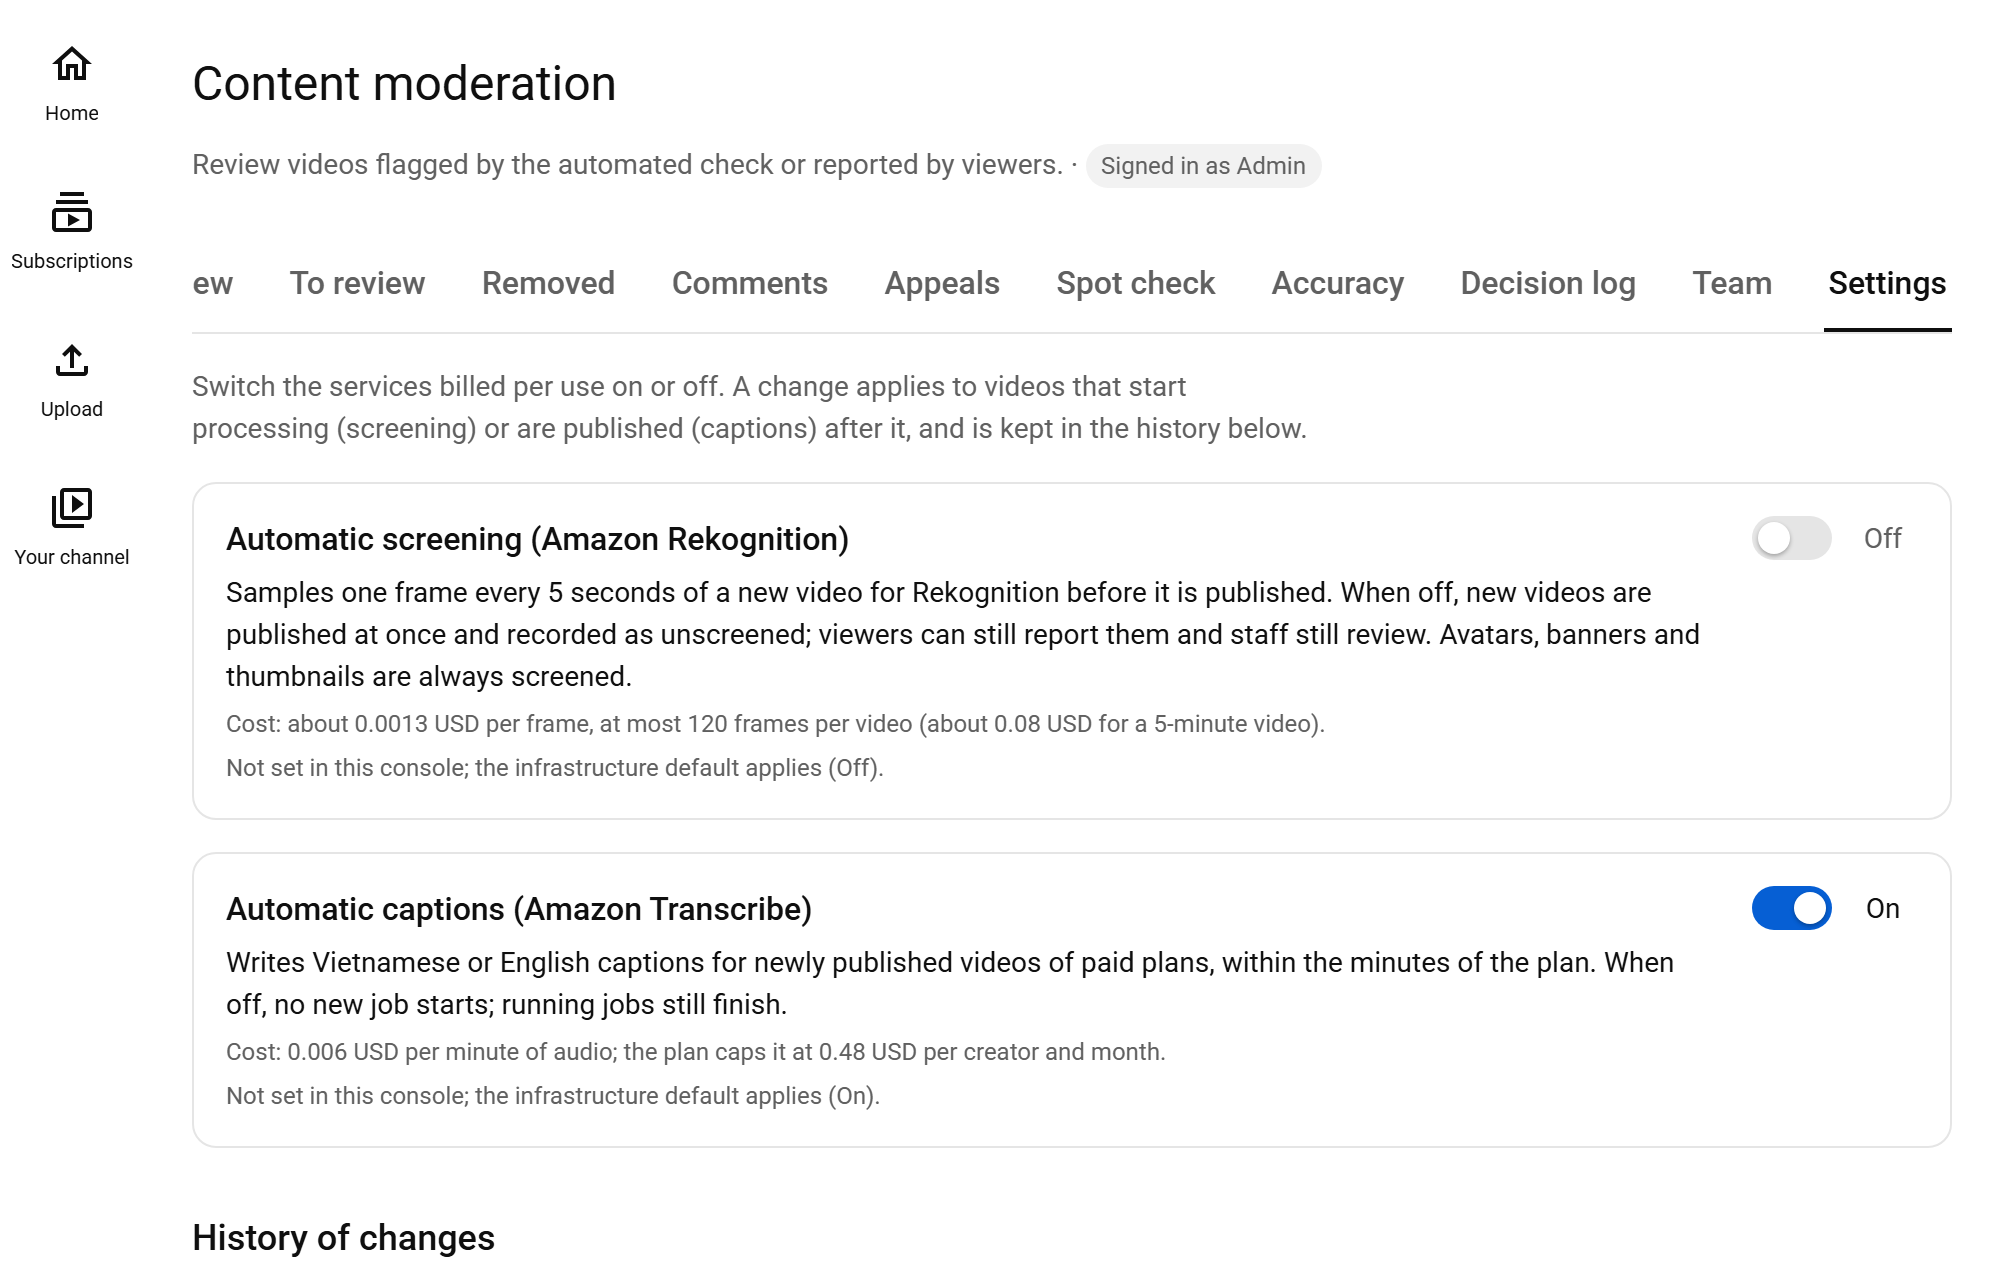
\includegraphics[width=\textwidth]{images/ui-admin-settings.png}
\caption{\textit{Settings tab of the staff console with the switches of screening and automatic captions}}
\label{fig:ui-settings}
\end{figure}
